\begin{frame}
\frametitle{\textbf{6.7.3.1 Formal definition of} \texttt{restrict}}
\begin{figure}
\centering
{
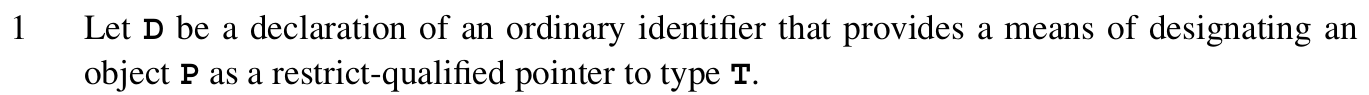
\includegraphics[width=0.9\textwidth]{restrict-definition-1.png}
}
{
\\
\qquad \vdots
\\
}
{
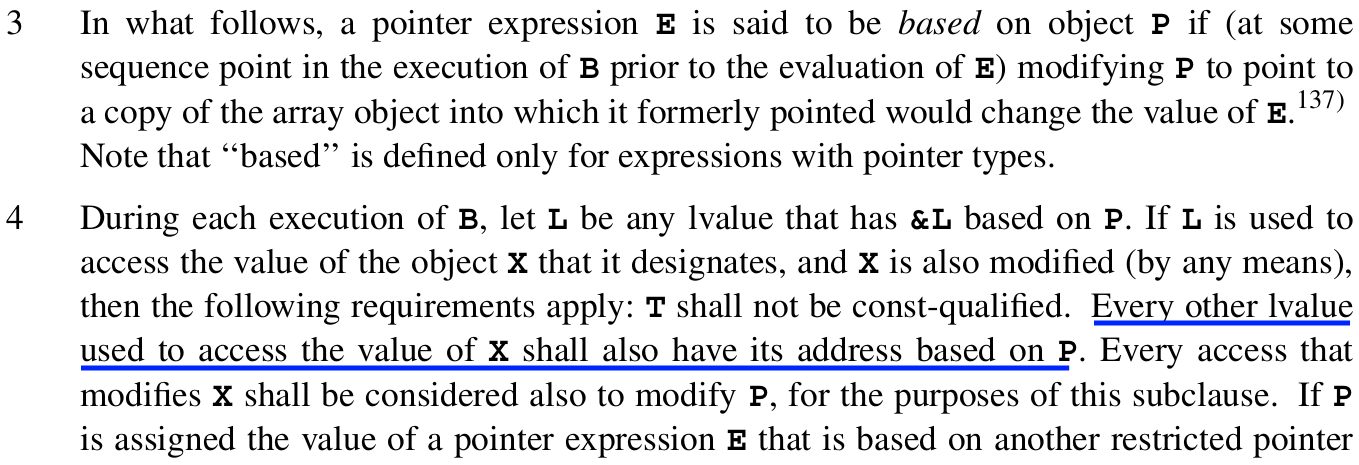
\includegraphics[width=0.9\textwidth]{restrict-definition-3-4-annotation-defined.png}
}
{
\\
\qquad \vdots
}
\end{figure}
\end{frame}

\begin{frame}
    \frametitle{\textbf{6.7.3.1 Formal definition of} \texttt{restrict}}
\begin{minipage}{0.5\textwidth}
\begin{itemize}
    \item Four N-documents submitted since 2018
    \item \setulcolor{red}\ul{Gustedt (2024)}\footnotemark: ``By its title it is a promise (to provide a formal definition) but it is in fact very delicate mix up of semantic concepts that make it almost impossible to comprehend from the given text.'' 
    \item MacDonald \etall (2022, 2024)\footnotemark \ report a bug in the definition of ``based on''
\end{itemize}
\end{minipage}%
\begin{minipage}{0.5\textwidth}
\begin{figure}
\centering
{
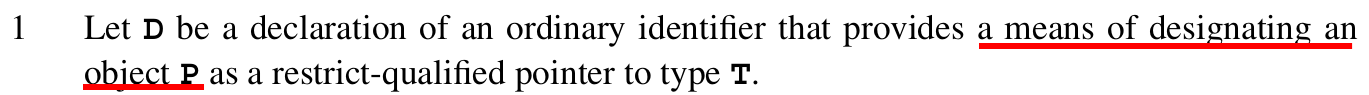
\includegraphics[width=0.95\textwidth]{restrict-definition-1-annotated.png}
}
{
\\
\qquad \vdots
\\
}
{
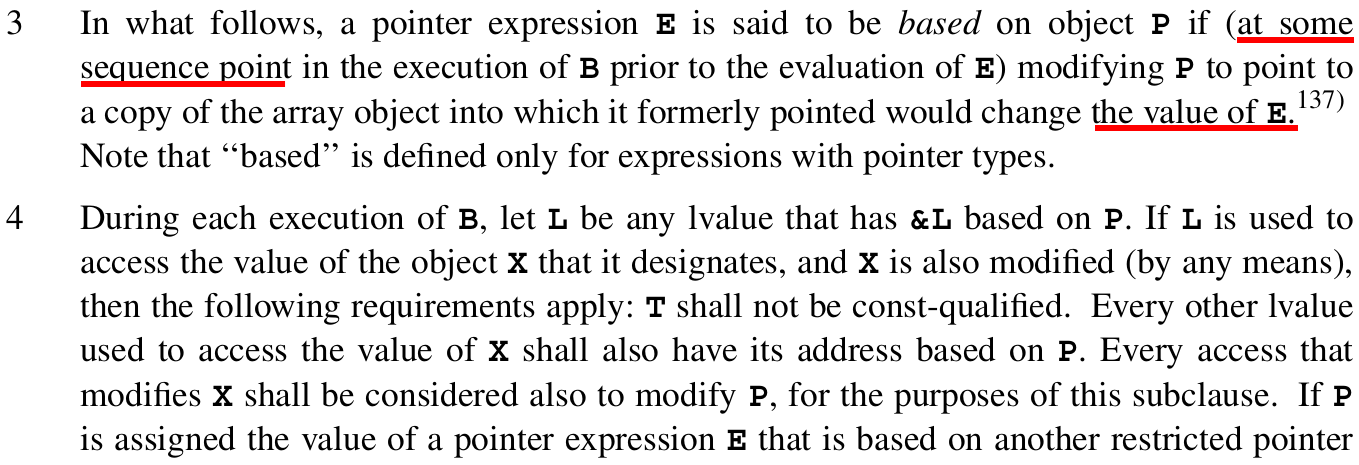
\includegraphics[width=0.95\textwidth]{restrict-definition-3-4-annotated.png}
}
{
\\
\qquad \vdots
}
\end{figure}
\end{minipage}

\footnotetext[1]{\cite{semanticsgustedt2024}}
\footnotetext[2]{\cite{defectmacdonald2022}} 

\end{frame}